% This document is compiled using pdfLaTeX
% You can switch XeLaTeX/pdfLaTeX/LaTeX/LuaLaTeX in Settings

\documentclass[b5paper, twoside]{article}
\usepackage{ctex}
\usepackage{csquotes} % 对于智能引用符号
\usepackage[backend=biber,style=numeric]{biblatex} % 使用biblatex和biber
\usepackage{geometry}
\usepackage{graphicx}
\usepackage{listings}
\usepackage{minted}
\usepackage{amsmath}
\usepackage{amsfonts}
\usepackage[T1]{fontenc}
\usepackage{lmodern}
\usepackage{amssymb}
\usepackage{marginnote}
\usepackage{xcolor}
\usepackage{hyperref}
\usepackage{todonotes}
\usepackage[utf8]{inputenc}
\usepackage{mdframed}
\usepackage{multicol}
\usepackage{url} % 加载url包
\usepackage[linesnumbered,ruled,vlined]{algorithm2e}
\usepackage{array} % 提供>{...}功能
\usepackage{booktabs} % 提供更好的表格线条
\usepackage{lipsum} % 用于生成占位文本
\usepackage{titlesec}
\usepackage{titling}
\usepackage{wrapfig}
\usepackage{enumitem}
\usepackage{parskip}
\usepackage{graphicx}
\usepackage{tikz}
\usepackage{newtxmath}
\usepackage{caption}
\usepackage{fancyhdr}  % 用于设置页眉和页脚
\usepackage{tocloft}  % 用于自定义目录
\usepackage{fontspec}
\setmainfont{Times New Roman}
% 设置 hyperref 的一些选项
\hypersetup{
	colorlinks=true,  % 使用颜色而不是框
	linkcolor=myblue,   % 内部链接的颜色
	urlcolor=cyan,    % URL 链接的颜色
	citecolor=green,  % 引用链接的颜色
	bookmarks=true,   % 创建书签
	pdfauthor={苏睿熹},  % 作者
	pdftitle={操作系统笔记},  % 标题
	pdfsubject={人工智能},  % 主题
}
% 设置目录标题
\renewcommand{\contentsname}{\textbf{目录与索引}}
% 调整各级标题的缩进
\setlength{\cftsecindent}{0em}  % 小节缩进
\setlength{\cftsubsecindent}{2em}  % 子小节缩进
\setlength{\cftsubsubsecindent}{4em}  % 子子小节缩进
% 调整各级标题的编号宽度
\setlength{\cftsecnumwidth}{2.5em}  % 小节编号宽度
\setlength{\cftsubsecnumwidth}{3.5em}  % 子小节编号宽度
\setlength{\cftsubsubsecnumwidth}{4.5em}  % 子子小节编号宽度
% 调整点线样式
\renewcommand{\cftsecleader}{\cftdotfill{\cftsecdotsep}}  % 小节点线
\renewcommand{\cftsubsecleader}{\cftdotfill{\cftsubsecdotsep}}  % 子小节点线
\renewcommand{\cftsubsubsecleader}{\cftdotfill{\cftsubsubsecdotsep}}  % 子子小节
%点线
% 设置点线间隔
\renewcommand{\cftsecdotsep}{\cftdot}  % 小节点线间隔
\renewcommand{\cftsubsecdotsep}{\cftdot}  % 子小节点线间隔
\renewcommand{\cftsubsubsecdotsep}{\cftdot}  % 子子小节点线间隔
% 设置字体样式
\renewcommand{\cftsecfont}{\bfseries}  % 小节字体
\renewcommand{\cftsubsecfont}{\bfseries}  % 子小节字体
\renewcommand{\cftsubsubsecfont}{\bfseries}  % 子子小节字体
% 设置页码字体样式
\renewcommand{\cftsecpagefont}{\bfseries}  % 小节页码字体
\renewcommand{\cftsubsecpagefont}{\bfseries}  % 子小节页码字体
\renewcommand{\cftsubsubsecpagefont}{\bfseries}  % 子子小节页码字体
% 设置页面布局
\pagestyle{fancy}
% 清除默认的页眉和页脚设置
\fancyhf{}
% 设置页脚
\fancyfoot[L]{苏睿熹}  % 左侧自定义文本
\fancyfoot[C]{操作系统笔记}  % 中间自定义文本
\fancyfoot[R]{跳转到\hyperref[toc]{目录}}  % 右侧自定义文本
% 设置页脚线的长度
\renewcommand{\footrulewidth}{0.4pt}  % 设置页脚线的粗细
\renewcommand{\headwidth}{\textwidth} % 设置页眉线的长度为文本宽度
% 设置页眉
\fancyhead[L]{\rightmark}  % 显示当前小节名称
\fancyhead[R]{\thepage}    % 显示页码
% 设置页眉线的长度
\renewcommand{\headrulewidth}{0.4pt}  % 设置页眉线的粗细
\renewcommand{\headwidth}{\textwidth} % 设置页眉线的长度为文本宽度
% 重新定义 \chaptermark 和 \sectionmark
\renewcommand{\sectionmark}[1]{\markright{\thesection\ #1}}
% 设置标题与图像之间的间距
\setlength{\abovecaptionskip}{5pt}  % 标题在图像上方的间距
\setlength{\belowcaptionskip}{0pt}  % 标题在图像下方的间距
\fvset{breaklines=true,
    frame=lines
}
\setlength{\parskip}{0pt}    % 设置段落之间的间距
\setlist[itemize,1]{left=0pt}
\setlist[itemize,2]{left=1pt}
\setlist[itemize,3]{left=1pt}
% 定义一个命令来设置图片的透明度
\let\oldincludegraphics\includegraphics
\renewcommand{\includegraphics}[2][]{%
  \begin{tikzpicture}
    \node[opacity=0.7] {\oldincludegraphics[#1]{#2}};
  \end{tikzpicture}%
}
% 设置页边距
\geometry{
    left=2cm,         % 左边距
    right=2cm,        % 右边距
    top=2.5cm,          % 上边距
    bottom=2.5cm        % 下边距
}
\lstset{
  language=Python,      % 语言类型
  basicstyle=\tt, %使用teletype字体
}
% 定义蓝色
\definecolor{myblue}{RGB}{0, 100, 225}
\definecolor{mypink}{RGB}{255,105,180}
% 重新定义 \maketitle 命令
\pretitle{\begin{center}\LARGE\bfseries\color{blue}}
\posttitle{\end{center}}
% 重定义 \textbf 命令
\let\oldtextbf\textbf
\renewcommand{\textbf}[1]{\textcolor{myblue}{\oldtextbf{#1}}}
% 重定义 \emph 命令
\let\oldemph\emph
\renewcommand{\emph}[1]{{\oldemph{#1}}}
\titleformat{\section}
  {\color{myblue}\bfseries\Large}
  {\thesection}
  {1em}
  {}
\titleformat{\subsection}
  {\color{myblue}\bfseries\large}
  {\thesubsection}
  {1em}
  {}
\titleformat{\subsubsection}
  {\color{myblue}\bfseries\normalsize}
  {\thesubsubsection}
  {1em}
  {}
% 定义一个带有较小字体的 mdframed 环境
\newenvironment{smallmdframed}
  {\begin{mdframed}[linewidth=0pt, backgroundcolor=pink!20]\small}
  {\end{mdframed}}

\title{操作系统笔记:中大2022人工智能学院课程}
\date{}

\begin{document}
	
\begin{minipage}[t]{\textwidth}
    \vspace{-0.5cm}
    \begin{center}
        \vspace{-1.5cm} % 减少间距
        
\includegraphics[width=0.2\textwidth]{img/sysu.jpg}\\
        \vspace{-1.5cm} % 减少间距
    \end{center}
    \maketitle
    \vspace{-4cm} % 减少间距
\end{minipage}
\vspace{-0.8cm}

\section{并发:死锁与饥饿}

\subsection{死锁原理}

死锁即一组相互竞争系统资源或者通信的进程“永久阻塞”。\\相互等待着被对方占有的共享资源,
共享资源可以分为可重用资源和可消耗资源。
\begin{itemize}
	\item {可重用资源}
	\begin{itemize}
		\item 
		\emph{可重用资源}指一次仅供一个进程安全使用且不因使用而耗尽的资源。\emph{重用}
		即重
		复使用。进程得到资源单元并使用后会释放供其他进程使用。
		\item 如:I/O通道、内存和外存、设备以及数据结构(文件、数据库和信号量)。
		\item 重用资源的竞争可能导致死锁。
	\end{itemize}
	\item {可消耗资源}
	\begin{itemize}
		\item \emph{可消耗资源}指可被创建和销毁的资源。
		\item 如:中断、信号、消息和I/O缓冲区的信息。
	\end{itemize}
\end{itemize}

\textbf{死锁与饥饿}
\begin{itemize}
	\item 死锁是进程在信号量内无穷等待,处于阻塞态。进程量大于1。
	\item 
	饥饿是由于分配策略不公平导致的进程长时间等待,处于阻塞态(等资源)或就绪态(等CPU)
	。发生饥饿的进程可以只有一个。
\end{itemize}

\textbf{死锁产生的原因}
\begin{itemize}
	\item 系统资源的竞争
	\item 进程推进顺序非法
\end{itemize}

\textbf{死锁产生的必要条件}:必须同时成立。\hfill{\emph{\textcolor{red}{significant}}}
\begin{itemize}
	\item \emph{互斥条件}:资源的排他性使用。
	\item \emph{不可剥夺条件}:不可以从其他进程中强行夺走其未释放的资源。
	\item 
	\emph{请求并保持条件}:保持资源时提出新的资源请求,请求不被满足时不释放保
	持资源。
	\item 
	\emph{循环等待条件}:
	\begin{itemize}
		\item 	存在进程资源的循环等待链,每个进程保持资源被链中的下一个进程所
		请求。
		\item 循环等待的条件比死锁弱,如下图所示。
		\begin{figure}[th]
			\centering
			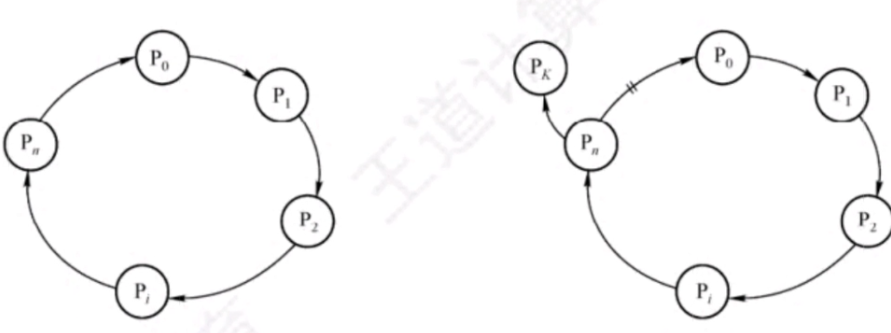
\includegraphics[width=0.7\linewidth]{img/ascreenshot001}
			\caption{循环等待的死锁与非死锁}
			\label{fig:ascreenshot001}
		\end{figure}
	\end{itemize}
\end{itemize}

\textbf{死锁的处理策略}
\\必须设法破坏产生死锁的四个必要条件,或有能力在死锁产生之后检测并回复。
\begin{itemize}
	\item \emph{死锁预防}:设置限制条件,破坏四个死锁必要条件。
	\item \emph{避免死锁}:在资源动态分配过程中防止系统进入不安全状态。
	\item \emph{死锁的检测与解除}:允许发生死锁,检测并接触死锁。
	\begin{figure}[th]
		\centering
		
\includegraphics[width=0.7\linewidth]{img/ascreenshot002}
		\caption{死锁处理策略比较}
		\label{fig:ascreenshot002}
	\end{figure}
\end{itemize}

\subsection{死锁预防}

\textbf{破坏互斥条件}:将只能互斥使用的资源改为允许使用的资源。

\textbf{破坏不可剥夺条件}:新的资源不被满足时,进程必须释放已经保持的所有资源。
\begin{itemize}
	\item 释放已经获得的资源可能导致前一阶段的工作失效。
	\item 一般适用于易保存和回复的资源,如CPU寄存器和内存资源。
\end{itemize}

\textbf{破坏请求并保持条件}:进程在请求资源的时候不能持有不可剥夺资源。
\begin{itemize}
	\item 
\end{itemize}

\tableofcontents

\appendix
\newpage

\section{附录1 Assignment}

\textbf{第四次作业}\hfill 苏睿熹 22330100
\begin{itemize}
	\item 习题6.6
	\begin{figure}[th]
		\centering
		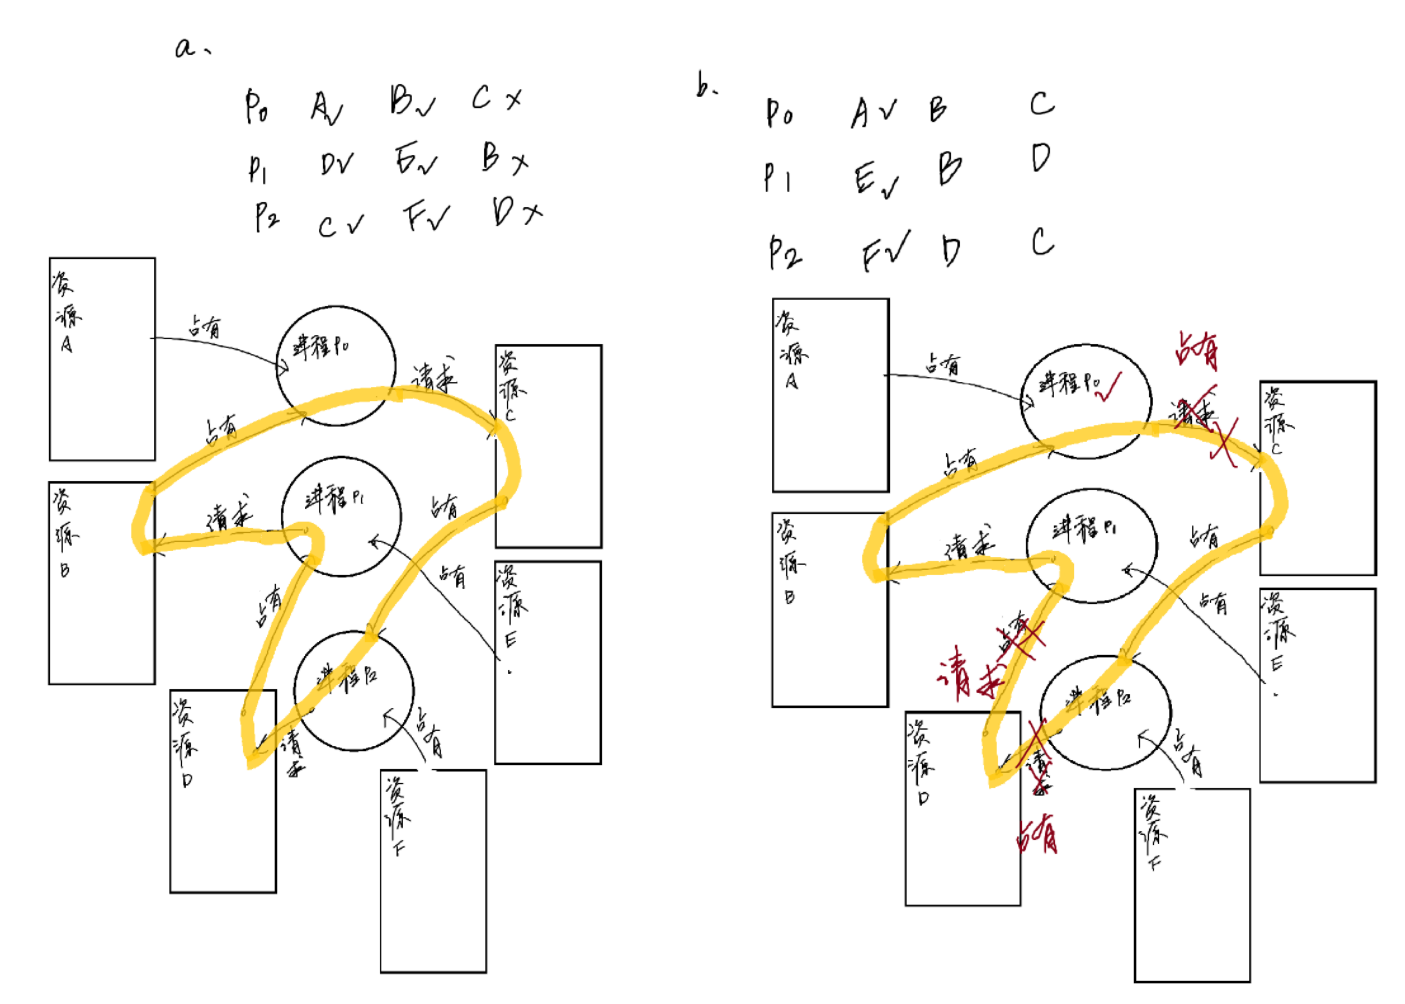
\includegraphics[width=0.7\linewidth]{img/ascreenshot003}
		\caption{习题6.6解答}
		\label{fig:ascreenshot003}
	\end{figure}
	\\调整后的资源请求顺序: 
	$P_0$:A$\Rightarrow$B$\Rightarrow$C;
	$P_1$:E$\Rightarrow$B$\Rightarrow$D;
	$P_2$:F$\Rightarrow$D$\Rightarrow$C

	\item 习题6.14
	\begin{itemize}
		\item[a. ] 
		会导致两个全部被阻塞。运行序列:\\\lstinline|foo.semWait(S)|$\rightarrow$\lstinline|bar.semWait(R)|
		$\rightarrow$\lstinline|foo.semWait(R)|$\rightarrow$\lstinline|bar.semWait(S)|
		\item[b. ] 可能会导致其中一个被无限期延后。运行序列:
		\begin{verbatim}
			foo.semWait(S); foo.semWait(R); x++;
			foo.semSignal(S); bar.semWait(R); foo.semSignal(R);
			foo.semWait(S); foo.semWait(R); x++;
			……
		\end{verbatim}
	\end{itemize}
	\item 习题6.15
	\begin{itemize}
		\item 目前已经分配的资源数量有:$1+1+3+2=7$,假设目前可用资源为$x\geq1$。
		\item 因为$x\geq1$,可执行$P_1$并释放。可用资源为$x+1\geq2$。
		\item 因为$x+1\geq2$,可执行$P_0$并释放,可用资源为$x+2$。
		\item 目前$P_2$和$P_3$分别需要6个和5个资源,优先执行$P_3$。
		\item 要使得$P_3$可执行,可用资源满足$x+2\geq5$。
		\item 释放$P_3$得可用资源为$x+4\geq7$,可执行$P_2$。
		\item 所以,要保证当前状态的安全性,最少需要$\min\{x\}+7=10$个单位的资源。
	\end{itemize}
	\item 习题7.5
	\begin{itemize}
		\item[a. ] \emph{优点}:最差适配算法倾向于选择最大的空闲存储块来放置进程。这
		样可以避免在较小的空闲块中留下大量的小碎片。通过使用较大的空闲块,减少了内部碎
		片的数量,从而提高了内存的整体利用率。\emph{缺点}:由于需要找到最大的空闲块,
		因此每次分配时都需要遍历整个可用内存列表,导致查找时间较长。如果频繁地为小进程
		分配大的空闲块,可能会导致大量未使用的内存被浪费。
		\item[b. ] 最差适配的平均查找长度取决于内存中的空闲块数量和大小分布情况。一般
		来说,由于每次分配都要遍历所有空闲块以找到最大的一个,所以平均查找长度会随着空
		闲块数量的增加而增加。
	\end{itemize}
	\item 习题7.12
	\begin{itemize}
		\item 逻辑地址有多少位?
		\[
		\text{逻辑地址} = \log_2(2^{32}) + \log_2(2^{10}) = 32 + 10 = 42 \text{ 
		bits}
		\]
		\item 一个页框有多少字节?
		\[
		\text{页框大小} = 2^{10} \text{ bytes} = 1024 \text{ bytes}
		\]
		\item 物理地址中有多少位是页框号?
		\[
		\text{物理地址} = \log_2(2^{32}) = 32 \text{ bits}
		\]
		\[
		\text{页框号} = \frac{\text{物理地址}}{\text{页框大小}} = \frac{32}{10} = 
		3.2 \approx 3 \text{ bits}
		\]
		\item 页表中有多少表项?
		\[
		\text{页表项数} = 2^{16}
		\]
		\item 假设每个页表项中含一位有效位,每个页表项有多少位?
		\[
		\text{页表项大小} = \log_2(2^{16}) + 1 = 16 + 1 = 17 \text{ bits}
		\]
	\end{itemize}
\end{itemize}


\label{toc}

\end{document}
